\chapter{Standard Suite}
Per riuscire a comuninicare fra nodi eterogenei in SW/HW sono necessari degli \textbf{standard}. I due principali sono:
\begin{itemize}
    \item \textbf{\textcolor{red}{ISO-OSI}.}
    \item \textbf{\textcolor{red}{TCP/IP}.}
\end{itemize}

\section{Modello ISO-OSI}
\begin{figure}[!htb]
    \centering
    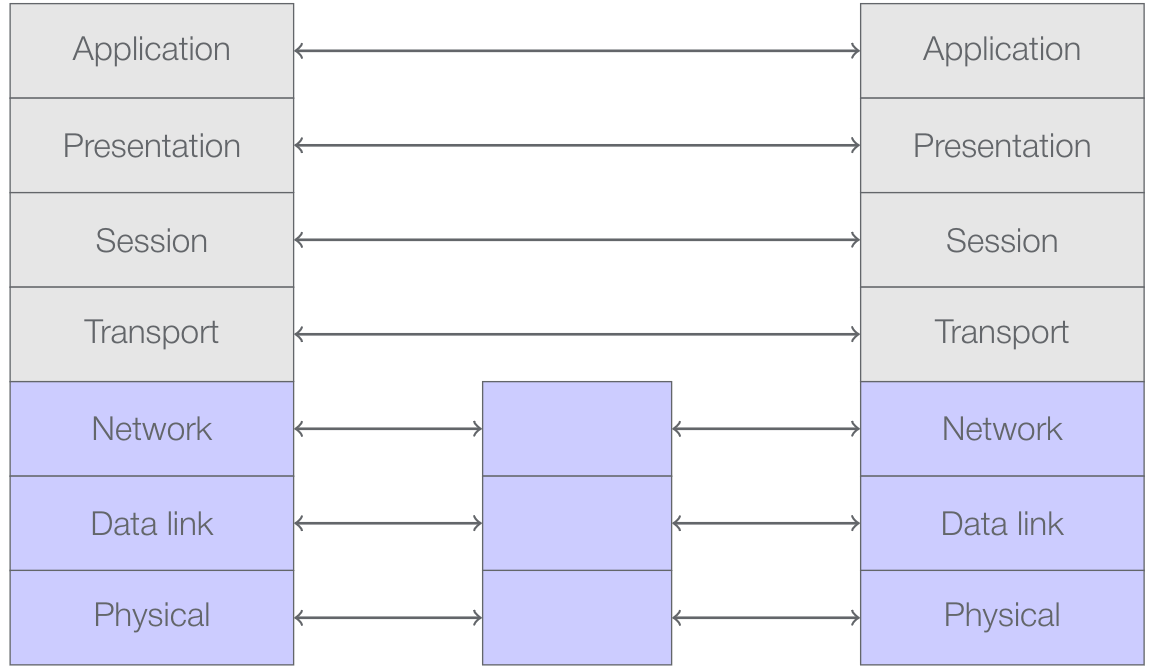
\includegraphics[width=0.6\linewidth]{Images/Standard_Suite/ISO-OSI_Stack.png}
    \caption{ISO-OSI Stack.}
    \label{fig:ISO-OSI}
\end{figure}

\begin{boxDef}
\textcolor{brown}{ISO (International Standard Organization):} defined the specifications of what should have become the protocol standard for the interconnection of heterogeneous nodes.
\\
\vspace*{0.001\textheight}
\\
\textcolor{brown}{OSI (Open Source Informaztion)}
\end{boxDef}

Lo stack \textbf{ISO-OSI} è formato da protocolli di \textbf{elaborazione} per gestire le applicazioni e da protocolli di \textbf{comunicazione} per gestire lo scambio di messaggi fra nodi di rete e per nascondere le caratteristiche del mezzo fisico di trasmissione. Ci sono in totale 7 livelli:
\begin{enumerate}
    \item \textbf{\textcolor{blue}{Fisico.}}
    \item \textbf{\textcolor{blue}{Data-Link.}}
    \item \textbf{\textcolor{blue}{Rete.}}
    \item \textbf{\textcolor{blue}{Trasporto.}}
    \item \textbf{\textcolor{blue}{Sessione.}}
    \item \textbf{\textcolor{blue}{Presentazione.}}
    \item \textbf{\textcolor{blue}{Applicazione.}}
\end{enumerate}

\subsection{Livello Fisico}
Gestisce i dettagli meccanici ed elettrici della trasmissione fisica di un flusso di bit.

\subsection{Livello Data-Link}
Gestisce frame o pacchetti trasformando la semplice trasmissione in una linea di comunicazione priva di errori non rilevati.

\subsection{Livello Rete}
Fornisce connessioni e instradamento dei pacchetti nella rete.

\subsection{Livello Trasporto}
Esegue il controllo end-to-end della sessione di comunicazione, accesso alla rete da parte del client e trasferimento di messaggi tra client.

\subsection{Livello Sessione}
Consente agli utenti su macchine eterogenee di stabilire sessioni, implementando le funzioni di coordinamento, sincronizzazione e mantenimento dello stato.

\subsection{Livello Presentazione}
Risolve le differenze di formato che possono sorgere tra i diversi nodi della rete e gestisce la compressione dei dati, la sicurezza e l'autenticità dei messaggi tramite tecniche di crittografia.

\subsection{Livello Applicazione}
Fornisce un'interfaccia standard per i programmi applicativi che utilizzano la rete, mascherando le peculiarità e la complessità del sistema sottostante.

\subsection{PDU dello stack ISO-OSI}
Ogni livello dello stack ISO-OSI aggiunge un header al PDU, che sarà formato quindi dalla informazioni e 7 header diversi.

\vspace*{0.03\textheight}
\begin{figure}[!htb]
    \centering
    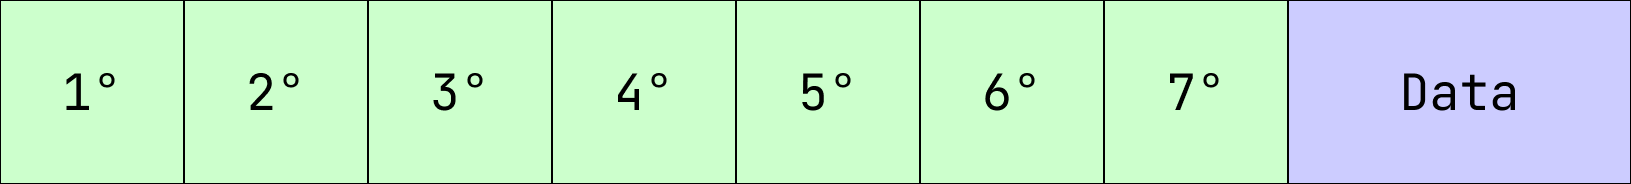
\includegraphics[width=0.7\linewidth]{Images/Standard_Suite/PDU_ISO-OSI.png}
    \caption{ISO-OSI PDU.}
\end{figure}

\newpage
\section{Modello TCP/IP}
\begin{figure}[!htb]
    \centering
    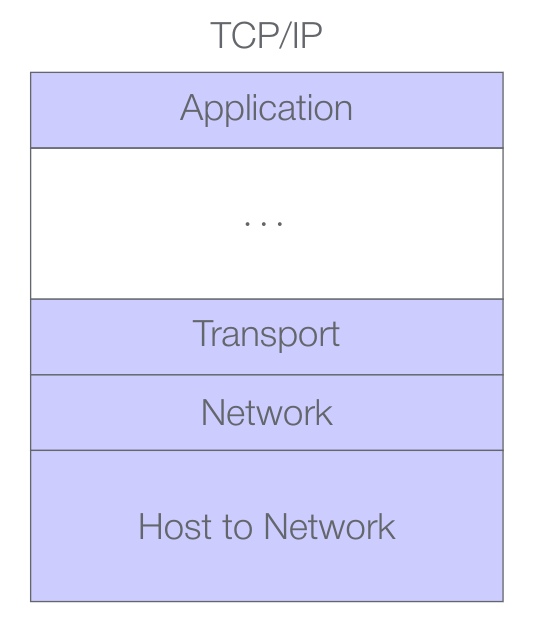
\includegraphics[width=0.3\linewidth]{Images/Standard_Suite/TCP-IP.png}
    \caption{TCP/IP Stack.}
\end{figure}

\textbf{TCP/IP} è il modello più usato ed è di fatto lo standard, anche perchè implementato nei sistemi UNIX e ha molte API per creare applicazione network. 

\subsection{Livello Host-to-Network}
Include i primi due livello del modello ISO-OSI che però rimangono indipendenti. Qui ci sono protoccoli com Ethernet, Token-Ring, 802.11, ecc...

\subsection{Livello Rete}
A questo livello viene usato il protocollo \textbf{IP}, che si occupa di mandare pacchetti dal un nodo sorgente a un nodo destinatario. Tratta ogni pacchetto indipendentemente e non assicura che tutto sia stato inviato correttamente.

\subsection{Livello Trasporto}
Si occupa del multiplezing e demultiplexing dei messaggi fra ogni processo e aggiunge un rilevamento degli errori.
I protocolli principali sono \textbf{TCP} e \textbf{UDP}.

\subsection{Livello Applicazione}
Il livello applicativo utilizza il livello di trasporto delle informazioni tra i processi in esecuzione sugli host terminali per creare applicazioni di rete. Alcuni protocolli usati sono \textbf{SSH}, \textbf{FTP}, \textbf{HTTP}, \textbf{SMTP}, ecc...

\section{Circuit switching}
Un circuito virtuale dedicato per ogni comunicazione, ha la necessità di riservare tutte le risorse end-to-end prima della trasmissione. Risorse dedicate e non è possibile la condivisione.
Ci sono due metodi per dividere le risorse:
\begin{itemize}
    \item \textbf{Frequency Based Methods (FDM).}
    \item \textbf{Time-based methods (TDM).}
\end{itemize}

\section{Packet Switching}
I dati vengono suddivisi in parti e inviati attraverso la rete.
Ogni pacchetto utilizza tutta la capacità di trasmissione di un collegamento. Le risorse vengono utilizzate in base alle necessità e non in base alla prenotazione.